%\documentclass{book}
%\usepackage{amsmath}
%\begin{document}
\section{Galaxy Cluster}
Galaxy clusters are the largest gravitationally bound objects in Universe. They mainly composed of galaxies (along with dust, stars and dust), hot gas clouds (30-100 million degree celsius) and invisible dark matter. The mass of the hot gas is 3-10 times greater than the mass determined from the visible luminosity of the galaxies. The total mass of cluster is typically $10^{14}\text{\,M}_{\odot}$ to  $10^{15.5}\text{\,M}_{\odot}$ (Seward F. D \& Charles P. A. 2010). The diameter is typically 2 to 10 Mpc and the velocity dispersion of the indivisual galaxies is about 400-1400 km\,s$^{-1}$. The fraction of galxies within cluster is $\sim$ 5$\%$ and contains 30-300 galaxies.\\\\
In clusters, the hot gas envelopes the galaxies and fill the space between galaxies. The hot gas contains more mass than the total galaxies. Scientists predicted that more mass about 10 times more than the hot gas and galaxies is required to hold the cluster together and this mass is given by mysterious dark matter.\\\\%%%%%%%%%%%%%%%%%%%%%http://chandra.harvard.edu/xray_sources/galaxy_clusters.html%%%%%%%%%%%%%%%%%%%%
The gas in the clusters is heated as the cluster is formed and such hot gases can be studied using X-ray spectra. During the evolution the hot gas and the dark matter in the cluster pushes the particles to the center of the cluster together. This causes them to collide and loose the energy by radiation. Ultimately after billions of year this hot gas looses energy and slowly settle onto a massive galaxy in the center of the clusters. Study of such flow is very useful to expalin the angular momentum orientation of galaxies.\\\\
Astronomers think that galaxy clusters form as clumps of dark matter and their associated galaxies are pulled together by gravity to form groups of dozens of galaxies, which in turn merge to form clusters of hundreds, even thousands of galaxies.\\\\%%%%%%%%%%%%%%http://www.astronomynotes.com/galaxy/s9.htm
The clustering process doesn't stop with galaxies. Galaxy clusters attaract each other to produce superclusters to tens to hundreds of clusters. The mutual gravitatioanl force binds the clusters and forms 300-900 millioin light year long, 150-300 million light year wide and 15-30 million light year thick on average. Voids can be found in intersupercluster medium, which are 150 million light year across, with very few galaxies.\\\\
Clusters can be classified as the open, globular and intermediate type clusters on the basis of potential energy and kinetic energy of the galaxies. Also, Bautz and Morgan has classified clusters on the basis of the morphology in 1970. It is mainly of three types I, II and III. Type I clusters is dominated by bright, large, supermassive cD galaxies, Type II contains elliptical galaxies whose brightness is intermediate of I and III and type III clusters has no remarkable members. 
\section{Two Degree Field Galaxy Redshifts Survey}
Two Degree Field Galaxy Redshifts Survey (2dFGRS) is a major spectroscopic survey taking the advantange of the capabalities of 2dF facility built by the Anglo-Australian Observatory. This survey has obtatined spectra of 245591 objects mainly galaxies. 2dFGRS has obtained the redshifts of 221414 galaxies as shown in figure \ref{2df}.
%include map of the galaxy distribution proudced from completed survey
\begin{figure}[H]
\begin{center}
 \includegraphics[height=6.9cm]{2dFzcone.eps}
        \caption{Galaxy distribution according to 2dFGRS.[source: web$^1$]}\label{2df}
        %http://www2.aao.gov.au/~TDFgg/
 \end{center}  
\end{figure}
\noindent The data from this survey is used to study the fundamental problems of galaxy formation and cosmology. An accurate measurement of power spectrum of galaxy clusters with precise determination of total mass density of universe and baryon fraction (Pervical et al. 2001), evidence of non-zero cosmological constant was also found combining the observation with cosmic microwave background (Efstathiou et al. 2002) and first direct measurement of the galaxy bias parameter, both from higher-order corrections in galaxy distribution (Verde et al. 2002) and from comparison with the CMB power spectrum (Lahav et al. 2002 ) are some of the results emerging from the survey.
\\
%%%%%%%%%%%%%%%%%%%%http://www.sdss.org/

\section{Sloan Digital Sky Survey}
Sloan Digital Sky Survey (SDSS) is most ambitious survey. It has covered more than a quarter of the sky and created 3-dimensional maps containing more than 930,000 galaxies and more than 120,000 quasars (Yanny B. et al. 2009). SDSS uses 2.5 m telescope at Apache Point observatory, New Mexico. A 120 megapixcel camera images 1.5 square degree of sky at a time and a pair of spectrographs measures the spectra of more than 600 galaxies and quasars in a observation.The three surveys that make up SDSS are:
\begin{itemize}
\item Legacy, imaging survey in five bands 7646 square degree high-altitude elliptical region in the Northern Galactic Cap,an additional 750 square degree in the Southern Galactic Cap, together with spectroscopy of complete samples of galaxies and quasars covering about 8200 square degrees.
\item SEGUE (Sloan Extension for Galactic Understanding and Exploration), images 3240 square degree at low Galactic latitude, together with spectroscopy of 240\,000 stars. 
\item Supernova, equivalent of about 80 repeated imaging scans of Southern Equatorial Stripe (ra$>$310 or ra $<$59; -1.25$>$dec$<$1.25) to search supernovae in the redshift range 0.1$<z<$0.4
\end{itemize} 
\begin{figure}[H]
\begin{center}
 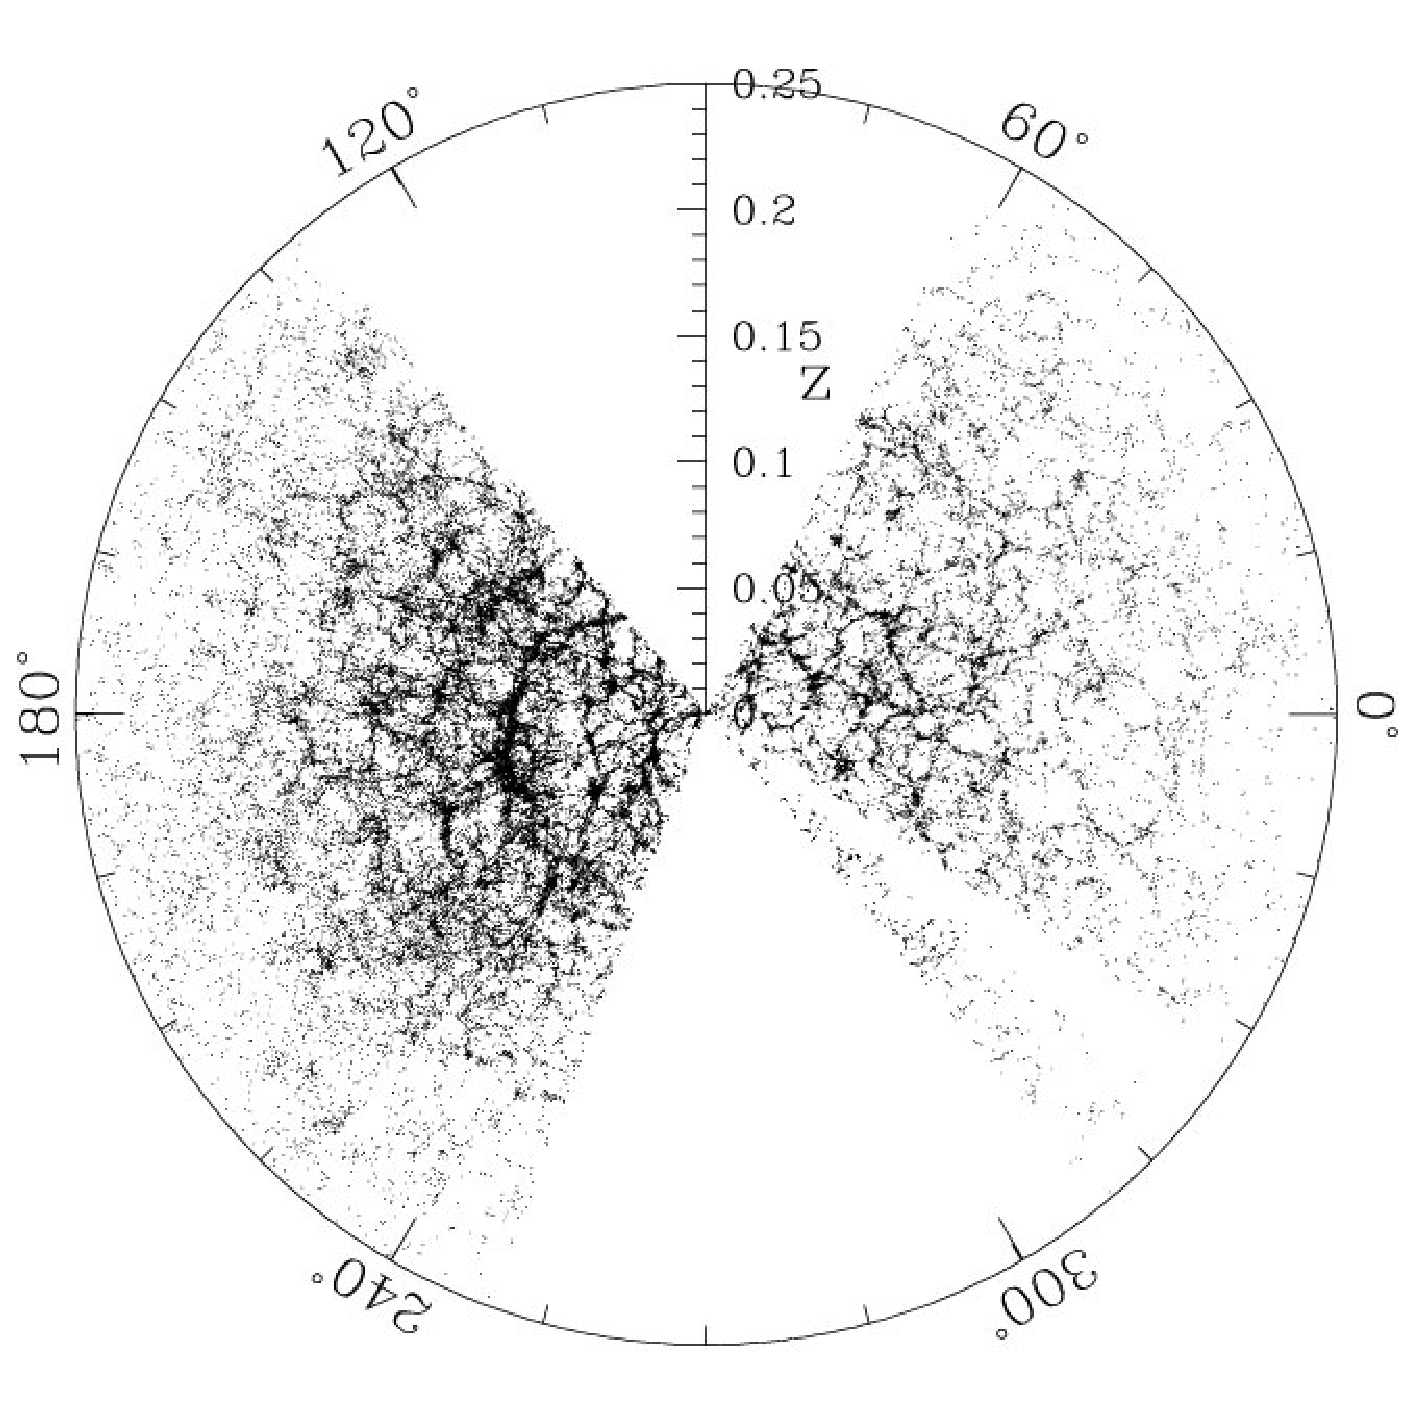
\includegraphics[height=7.5cm]{SDSS.eps}
        \caption{SDSS Spectroscopic Survey Shows Spongy Distribution of Galaxies in the Universe.[source: web$^2$]}\label{SDSS}
        %http://www.fnal.gov/pub/today/archive/archive_2005/today05-05-04.html
 \end{center}  
\end{figure}
\noindent During its first phase operations, 2000-2005, the SDSS imaged more than 8000 square degrees of the sky in five optical bandpasses, and it obtained spectra of galaxies and quasars selected from 5700 square degrees of that imaging. The seventh data relese DR7 imaging data covers about 8423 square degree of  legacy sky and 3240 square degrees fo SEGUE sky. DR7 includes more than 350 million celestial objects and spectra of 930000 galaxies,120,000 quasars and 460,000 stars.\\\\
One of the burning question of the modern astronomy is the problem of origin of angular momentum of the galaxies during their formation. It is interesting and challenging problem to cosmology as well.
%\subsubsection{Primodial Vorticity model:}
%This moel predicts that the spin vectors of galaxies are distributed perpendicular to the cluster plane. The primordial vorticity is called top-down scenario. Sometimes it is also called turbulence model. In the turbulence scenario, an initial large-scale vorted in the protocluste with intinsic vortex is formted and this vorted is fragmented into severl pieces with form teh bsis for the protogalaxies and the galaxies later on.So, the galactic spin vectors are thought to be parallel among themselves and perpendicular to the plane of the cluster.
%
%Ozernoy (1971, 1978) proposes that galaxies form from high-density regions behind the shocks produced by turbulence. According to the primordial vorticity theory, the presence of large chaotic velocities generates turbulence, which, in turn, produces density and pressure fluctuations.
%
%Density fluctuations on the scale of clusters of galaxies could be gravitationally bound, but galactic mass fluctuations are always unbound. Galaxies form when unbound galactic mass eddies, expanding faster than their bound cluster background. So forming galaxies collide with each other as clusters start to recollapse. These collisions produce shocks and high-density proto-galaxies at the eddy interfaces. As clusters recollapse, the system of galaxies undergoes a violent collective relaxation.
%
%
%\subsubsection{Pancake Model}
%The pancake model was first proposed in the 1970s by Yakob B. Zel'dovich at the Institute of Applied Mathematics in Moscow.
%
%The pancake model predicts that the spin vectors of galaxies tend to lie within the cluster plane. In the pancake scenario, formation of clusters took place first and it was followed by their fragmentation into galaxies due to adiabatic fluctuations. According to the non-linear gravitational instability theory, a growth of small inhomogeneities leads to the formation of thin, dense, and gaseous condensations that are called `pancakes'. These condensations are compressed and heated to high temperatures by shock waves causing them to quickly fragment into gas clouds. The later clumping of these clouds results in the formation of galaxies and their clusters.
%
%Thermal, hydrodynamic, and gravitational instabilities arise during the course of evolution. It leads to the fragmentation of gaseous proto-clusters and, subsequently, clustering of galaxies takes place. The pancake scheme follows three simultaneous processes: first, gas cools and new clouds of cold gas form; secondly, these clouds cluster to form galaxies; and thirdly, the forming galaxies and, to an extent, single clouds cluster together to form a cluster of galaxies.
%
%\subsubsection{Hierarchy Model}
%According to the hierarchy model, the directions of the spin vectors should be distributed randomly. In hierarchy model, galaxies were first formed and then they obtained their angular momenta by tidal force while they were gathering gravitationally to form a cluster. Those galaxies grow by subsequent merging of proto-galactic condensations or even by merging of already fully formed galaxies. In this scheme, one could imagine that large irregularities like galaxies grew under the influence of gravities from small imperfections in the early universe.
%
%The angular momentum transferred to a developing proto-galaxy by the gravitational interaction of the quadrupole moment of the system with the tidal field of the matter.
Some people found and discussed similarity of spiral galaxies to turbulent eddies and suggested that the primordial turbulence is respbonsible for the formation of galaxies and may be the origin of the rotation of galaxies (Weizacker 1951 , Gamow 1946). But this model fails because primodial turbulence cannot provide the angular momentum to the galaxies for long time as it dissipates (Jones and Peebles 1972, Jones 1973). Also there is another proposal that the galaxies acquire their angular momentum by the tidal torques of neighbouring protogalaxies (Hoyle 1951, Peebles 1969). But it was unable to explain the empirical relation between angular momentum and mass of the galaxy J$\propto M^{\frac{5}{3}}$ (Barres \& Efstahiou 1987). But in the scenario of global rotation of universe (Li 1998), the corollis force in the galactic frames make galaxies to rotate automatically when they form and galaxies get angular momentum from global rotation of universe due to conservation of angular momentum. So, galaxies rotate because universe rotate.
\section{Theoretical Consideration}
Li explained the empirical relation taking the help of Raychaudhari equation (Ciufolini \& Wheeler 1995) and Einstein field equation (Weinberg 1972).
\subsection{Raychaudhari Equation}
To study the properties of the rotating cosmological model we must define some of the terms like volume scalar expansion, shear tensor and rotation tensor. Raychauduri equation is the connection between these and Ricci curvature tensor.\\\\
Let us consider a ideal fluid whose four velocity $u^\alpha=\frac{dx^\alpha}{ds}$, where $s$ is the parameter of arc length and $x^\alpha\equiv x^\alpha(s)$. And four velocity satisfies the equation
\begin{equation}\label{g_ab}
g_{\alpha\beta}u^\alpha u^\beta=-1
\end{equation}
We can decompose any vector to time like component and space like components by applying a time projection tensor ($-u_\alpha u_\beta$) and space projection tensor $h_{\alpha\beta}=g_{\alpha\beta}+u_\alpha u_\beta$\\
Here,
\begin{eqnarray}\label{projection_time_space}
P_t(v^\alpha)&=&-u_\alpha u_\beta v^\beta\\
P_\Sigma(v^\alpha)&=&h_{\alpha\beta}v^\beta
\end{eqnarray}
Now the length element is given by,
\begin{eqnarray*}
ds^2&=&g_{\alpha\beta} dx^\alpha dx^\beta\\
&=&(h_{\alpha\beta} -u_\alpha u_\beta)dx^\alpha dx^\beta
\end{eqnarray*}
\begin{equation}
ds^2=h_{\alpha\beta}dx^\alpha dx^\beta -u_\alpha u_\beta dx^\alpha dx^\beta
\end{equation}
Let us consider, an observer in $x^\alpha$ which is comoving with the fluid particle with four velocity $u_\alpha$ measures two events $x^\alpha$ and $x^\alpha+dx^\alpha$ at space interval $dl=(h_{\alpha\beta}dx^\alpha dx^\beta)^\frac{1}{2}$ and time interval $d\tau=(u_\alpha u_\beta dx^\alpha dx^\beta)^\frac{1}{2}$\\\\
\textbf{Some properties of $h_{\alpha\beta}$:}
\begin{equation}
\begin{aligned}
h_{\alpha\beta}u^\beta&=&0\hspace{1cm}h_{\alpha\beta}\dot{u}^\beta=h_{\alpha\beta}\underbrace{u^\beta_{;\sigma}u^\sigma}_{\mbox{$a^\beta$}}=h_{\alpha\beta}a^\beta=a_\alpha\\
h^{\alpha\beta}h_{\beta\gamma}&=&h_{\gamma}^{\alpha}\hspace*{1cm} h_{\alpha}^\alpha =3
\end{aligned}
\end{equation}
where $a^\alpha$ is four accleration of fluid particles.\\
Now decomposing $u_{\alpha ;\beta}$ into space like and time like components using projection tensors
\begin{eqnarray*}
u_{\alpha ;\beta}&=& u_{\mu ;\nu}g^\mu_\nu g^\nu_\beta\\
&=& u_{\mu ;\nu}(h^\mu_\alpha-u^\mu u_\alpha)(h^\nu_\beta-u^\nu u_\beta)\\
&=& u_{\mu;\nu}h^\mu_\alpha h\nu_\beta -u_{\alpha;\nu} u^\nu u_\beta
\end{eqnarray*}\\
So the time and space component of  $u_{\alpha ;\beta}$ is given
\begin{equation}\label{u_a_b}
u_{\alpha ;\beta}=u_{\mu;\nu}h^\mu_\alpha h\nu_\beta -u_{\alpha;\nu} u^\nu u_\beta
\end{equation}
Let us introduce three quantities that helps to describe rotating cosmological model:
\begin{itemize}
\item The scalar $\Phi$ of volume expansion\begin{equation}
\Phi=u^\alpha_{;\alpha}
\end{equation}
\item Traceless symmetric tensor of shear:
\begin{equation}
\sigma_{\alpha\beta}=\left[u_{(\mu;\nu)}-\frac{1}{3}\Phi h_{\mu\nu}\right]h^\mu_\alpha h^\nu_\beta$$
\end{equation}
\item The anti-symmetric tensor of vorticity:
\begin{equation}
\omega_{\alpha\beta}=u_{[\mu;\nu]}h^\mu_\alpha h^\nu_\beta
\end{equation}
\end{itemize}
where; $$u_{(\mu;\nu)}=\frac{1}{2}\left(u_{\mu;\nu}-u_{\nu;\mu}\right)$$
$$u_{[\mu;\nu]}=\frac{1}{2}\left(u_{\mu;\nu}+u_{\nu;\mu}\right)$$
Note: \\$a^\beta u_\beta=\sigma_{\alpha\beta}u^{\beta}=\omega_{\alpha\beta}u^{\beta}=0$
\\\\
Using the defined quantities $\Phi$, $\omega_{\alpha\beta}$ and $\sigma_{\alpha\beta}$ we can write \eqref{u_a_b} as,
\begin{equation}\label{phi_sig_ome}
u_{\alpha ;\beta}=\sigma_{\alpha\beta}+\omega_{\alpha\beta}+\frac{1}{3}\Phi h_{\alpha\beta}-a_\alpha a_\beta
\end{equation}
In the above expression $\Phi$, $\omega_{\alpha\beta}$ and $\sigma_{\alpha\beta}$ represents the decompositon of space-space projection of $u_{\alpha ;\beta}$ into trace of symmetric part, antisymmetric part and symmetric traceless part.\\\\
In general, the scalar of expansion $\Phi$ repesents the fractional rate of volume expansion of local ensemble of fluid particles, the shear tensor $\sigma_{\alpha\beta}$ represents the distortion in the generic local fluid ensemble at constant volume and the vorticity tensor $\omega_{\alpha\beta}$ represents the rotation of the generic local ensemble of fluid particles with respect to gyroscope.\\\\
From the tensor analysis we have;
\begin{equation}\label{riemann}
u_{;\mu;\nu}^\alpha-u_{;\nu;\mu}^\alpha=R^\alpha_{\sigma\nu\mu}u^\sigma
\end{equation}
Contracting $\alpha$ and $\nu$ in \eqref{riemann} and multiplying with $u^\mu$ we get;
\begin{equation}\label{R}
u_{;\mu;\alpha}^\alpha u^{\mu}-u^{\alpha}_{;\alpha;\mu}u^{\mu}=R_{\sigma\mu}u^{\sigma}u^{\mu}
\end{equation}
From \eqref{phi_sig_ome} and \eqref{R} we get;
\begin{equation}\label{Raychudhari_0}
\dot{\Phi}-\dot{u}^\alpha_{;\alpha}+2(\sigma^2-\omega^2)+\frac{1}{3}\Phi^2 =-R_{\alpha\beta}u^\alpha u^\beta
\end{equation}
where $\dot{A}^\beta=A^\beta_{;\sigma}u^\sigma$, $\sigma^2=\frac{1}{2}\sigma_{\alpha\beta}\sigma^{\alpha\beta}$, $\omega^2=\frac{1}{2}\omega_{\alpha\beta}\omega^{\alpha\beta}$ and $R_{\alpha\beta}$ is the Ricci Tensor.\\\\
Einstein field equation is given by
\begin{equation}\label{eins}
R_{\mu\nu}-\frac{1}{2} R g_{\mu\nu}= 8\pi T_{\mu\nu}
\end{equation}
Since we are considering perfect fluid the stress energy tensor of the fluid is
\begin{equation}\label{stess}
T_{\mu\nu}=(\rho+p)u_\mu u_\nu -pg_{\mu\nu}
\end{equation}
where $\rho$ and $p$ is the density and pressure of the perfect fluid.
From \eqref{eins} and \eqref{stess} we can find;
\begin{equation}\label{Rab_p_rho}
R_{\mu\nu}u^\mu u^\nu=4\pi(\rho +3p)
\end{equation}
Using \eqref{Rab_p_rho} in \eqref{Raychudhari_0} we get Raychaudhuri equation
\begin{equation}\label{Raychaudhuri}
\dot{\Phi}+\frac{1}{3}\Phi^2+2(\sigma^2-\omega^2)-a^\alpha_{;\alpha}=-4\pi(\rho +3p)
\end{equation}
When particle follows geodesic $a^\alpha=0$. So,
\begin{equation}\label{dust}
\dot{\Phi}+\frac{1}{3}\Phi^2+2(\sigma^2-\omega^2)=-4\pi(\rho +3p)
\end{equation}
From Robertson-Walker (R-W) metric and defination of $\Phi$ we have,
\begin{equation}
\frac{\Phi(t)}{3}=\frac{\dot{R(t)}}{R}=H
\end{equation}
The conservation of energy and momentum (Ellis 1973) gives;
\begin{equation}
\dot{\rho}=-(\rho+p)\Phi\quad\quad\quad \omega\rho a^5= \text{constant}
\end{equation}
We know form R-W metric, for dust $\rho_d\propto a^{-3} $and for radiation $\rho_r\propto a^{-4}$. So, $\omega_d\propto a^{-2}$ and $\omega_r\propto a^{-1}$. But the shear $\sigma$ falls off as $\sigma \propto a^{-3}$\\\\
For dust fluid $a^\alpha=0$, since it follows the geodesic and neglecting the shear term as it is assumed to be small. Then the first integral of \eqref{dust} gives
\begin{eqnarray*}
\dot{\Phi}+\frac{1}{3}\Phi^2-2(\omega^2)&=&-4\pi(\rho +3p)\\
\dot{\Phi}+\frac{1}{3}\Phi^2-2(\omega^2)&=&-4\pi(\rho)\quad\text{(p=0 for dust)}\\
\end{eqnarray*}
And \begin{equation}\frac{\Phi}{3}=H=\frac{\dot{a}}{a}\end{equation} Then, the first integral gives;
\begin{equation}\label{RW_r}
H^2=\frac{8\pi}{3} G\rho-\frac{2}{3}\omega^2-\frac{k}{a^2}
\end{equation}
where k is the integration constant and its value can be +1, 0, -1 by rescaling.\\
We can see \eqref{RW_r} is same as explained by R-W metric adding a centrifugal term due to rotation of the universe.
\subsection{Derivation of Empirical Formula $J\propto M^\frac{2}{3}$}
Let us consider formation of galaxies in rotating and expanding universe. At some early epoch there is density fluctuation in a region then the expansion around the region began to increasily decelerated.\\\\
Let us assume the density fluctuation be spherically symmetric. The region containing the proto-galaxy or matter which will turn galaxy in future is sphere (approximately due to the spherically symmetric density fluctuation).\\\\
Let at that epoch angular momentum relative to the gyroscopic frame be
\begin{equation}\label{J-i}
J_i=\frac{2}{5}M r_i^2 \omega_i
\end{equation}
where $M$ is the mass of the proto galaxies, $r_i$  is the radius of the proto-galaxy and $\omega_i$ is the angular velocity of the universe.\\\\
Again, we can also define a local frame called galactic frame axis which corotate with the global rotation of universe and its origin is fixed at galactic center. This is the frame with which the measurement is taken in real life.\\\\
After the formation of the galaxy, it rotates relative to the galactic frames which is caused by the corollis force or conservation of the angular momentum. At any epoch after the galaxy has formed, its angular momentum relative to the gyroscopic frame is given by
\begin{equation}\label{J-f}
J_f=J+\beta M r_f^2 \omega_f
\end{equation}
where $\omega_f$ is angular velocity of universe at present, $\beta$ is the parameter that depends on the distribution of mass in galaxy, $r_f$ radius of the galaxy at present and $J$ is the angular momentum of the galaxy relative to the galactic frame.\\\\
Also we know that,
\begin{equation}\label{om_rh_m}
\begin{aligned}
\omega_i=\omega_0(1+z_i)^2\\
\rho_d=\rho_{d0}(1+z_i)^3\\
M=\frac{4}{3}\pi\rho_{di}r_i^3
\end{aligned}
\end{equation}
From \eqref{J-i}, \eqref{J-f}, \eqref{om_rh_m} and using law of conservation of angular momentum we get,
\begin{eqnarray*}
J_i&=&J_f\\
\frac{2}{3}M r_i^2 \omega_i &=&  J+\beta M r_f^2 \omega_f\\
\end{eqnarray*}
Finally,
\begin{equation}\label{Jexp}
J=\frac{2}{5}\left(\frac{3}{4\pi\rho_{d0}}\right)^\frac{2}{3}\omega_0 M^\frac{5}{3}-\beta r_f^2(1+z_f)\omega_0 M
\end{equation}
For $z_f$ not too large than 1, second term in \eqref{Jexp} is sufficiently small compared to first term so
\begin{gather*}
J\simeq k M^\frac{5}{3}\\
\text{where} \quad k=\frac{2}{5}\left(\frac{3}{4\pi\rho_{d0}}\right)^\frac{2}{3}\omega_0
\end{gather*}
and this explains the observed empirical relation $J\propto M^\frac{5}{3}$
\subsection{Limiting Value of Angular Momentum}
Minimizing \eqref{Jexp} with respect to M we get,
\begin{eqnarray*}
\frac{dJ}{dM}\rfloor_{M_{min}}&=&0\\
&=&\frac{d}{dM}\left(k M^\frac{5}{3}-l M\right)\rfloor_{M_{min}}\quad \text{where $l=\beta r_f^2(1+z_f)^2\omega_0$}\\
&=&k\frac{5}{3}M_{min}^{\frac{2}{3}}-l
\end{eqnarray*}
\begin{equation}
M_{min}=\left(\frac{3l}{5k}\right)^{\frac{3}{2}}=1.95 r_f^3 (1+z_f)^3 \rho_{d0}
\end{equation}
Hence the mininum angular momentum of a galaxy corresponds to the value of mass $1.95 r_f^3 (1+z_f)^3 \rho_{d0}$

\subsection{Zero Angular Momentum}
From \eqref{Jexp} we get,
\begin{eqnarray*}
J&=&0\\
 \text{or, }k M^\frac{5}{3}&=&lM\\
 \therefore \quad\quad M=\left(\frac{l}{k}\right)^\frac{3}{2}
 \end{eqnarray*}
 
\noindent Hence, the mass corresponding to the 0 angular momentum of galaxy is  $M_0\simeq 2.15 M_{min}$. It is easy to observe that for less and more massive structure predicts $\mid J\mid \neq 0$.\\\\
Till here it was concluded that the galaxy obtained its angular momentum due to the global rotation of the universe. So, one may expect that the spin of galaxies should not distribute in sky randomly, there should be a dipole anisotropy and such kind of anisotropy in the distribution of the spin of galaxies have been found at different levels. Here spherical symmetry is considered but the distribution of galaxy is quiet complicated and moment of inertia is complex so the angular momentum is different from the direction of angular velocity.\\\\
When proto-galaxy rotates and expands together with universe the angular velocity is equal to the global rotation of the universe in both magnitude and direction. The rotation of the universe makes the angular momentum of the protogalaxy which is not alligned with the angular velocity with a fixed direction to precesss about axis of rotation. The magnitude of angular momentum is constant during precission. When the proto-galaxies become separated from the global rotation and expansion of the universe and begins to collapse to form galaxies and the interaction with the surrounding should become more and more weak and eventually negligible. Its angular momentum is constant in both magnitude and direction. It should be determined by the shape of the proto-galaxy and the time when proto-galaxy becomes an isolated system. Its distribution can be expected  almost random instead of strong dipole distribution. As the galaxy evolves the dissipation process inside it causes the components of angular velocity perpendicular to the angular momentum to vanish gradually, eventually the galaxy rotates about the direction of angular momentum.
%\end{document}